%=========================================================================
% (c) 2014, 2015 Josef Lusticky

\section{Multiqueue adapters and scaling}\label{sec:linux-scaling}
One of the fundamental data structures in the networking subsystem is the transmit queue associated with each device.
As described in section~\ref{sec:linux-egress}, the core networking code will call the driver's {\it{ndo\_start\_xmit()}}
function to let the driver know that a packet is ready for transmission~\cite{mq-networking}.
The driver feeds that packet into hardware's transmit queue,
which results in a data structure which is shown in figure~\ref{fig:linux-queue-old}.
\begin{figure}
	\centering
	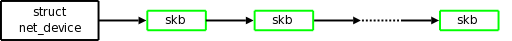
\includegraphics[width=11cm,keepaspectratio]{fig/net-queue-old.png}
	\caption{Single queue device (source:~\cite{mq-networking})}
	\label{fig:linux-queue-old}
\end{figure}

This scheme has worked well for years, but it does not map well to devices which have multiple transmit queues.
The multiqueue devices need each transmit queue to be scheduled independently.
10 and 40~Gigabit Ethernet devices with multiple transmit queues are very common~\cite{mq-networking}.

To provide an independent scheduling of a transmit queue,
a new {\it{netdev\_queue}} structure is implemented in the Linux kernel.
The {\it{netdev\_queue}} structure encapsulates all of the information about a single transmit queue,
and it is protected by its own lock.
Multiqueue device drivers set up an array of these structures according to the number of queues.
The {\it{mq}} (multiqueue) queueing  discipline uses the array to attach a specific {\it{qdisc}} to each queue.
The {\it{mq}} discipline is a dummy scheduler, which is used by default
for multiqueue devices instead of the regular {\it{pfifo\_fast}} discipline~\cite{kernel-doc-multiqueue}.
Figure~\ref{fig:linux-queue-mq} shows the new data structure.
\begin{figure}
	\centering
	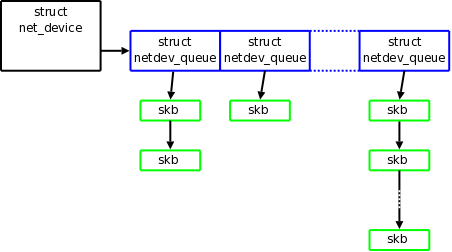
\includegraphics[width=11cm,keepaspectratio]{fig/net-queue-mq.png}
	\caption{Multiqueue device (source:~\cite{mq-networking})}
	\label{fig:linux-queue-mq}
\end{figure}

In addition to multiple transmit queues,
modern high-speed network adapters support multiple receive queues as well~\cite{mellanox-product-brief}.
The principle described above also applies to the receive queues in the Linux kernel.
The multiqueue support allows to scale the network load in multiprocessor systems.
Such scaling is provided by processing each queue by a different CPU~\cite{kernel-doc-scaling}.
The NIC distributes packets to the queues by applying a filter that assigns each packet to one of the receive queues.
The filter is a hash function (usually Toeplitz hash algorithm) over the network and transport layer headers of the packet
and a hash key, which is stored in the NIC's memory.
This mechanism is generally known as Receive Side Scaling (RSS)
and its goal is to increase performance uniformly~\cite{kernel-doc-scaling}.

Network adapters that do not support RSS but have multiple receive queues can still benefit from multiprocessor scaling
by using Receive Packet Steering (RPS), which is a software implementation of RSS~\cite{kernel-doc-scaling}.
However, there are some disadvantages of RPS against the hardware-based RSS.
The calculation of the hash requires accessing data from the packet header.
That access will necessarily involve one or more cache misses on the CPU running the RPS code -
that data was just put there by the network interface and thus cannot be in any CPU's cache~\cite{receive-packet-steering}.
Once the packet has been passed over to the CPU which will be doing the real work,
that cache miss overhead is likely to be incurred again.
Moreover, the targeted CPU is notified by an inter-processor interrupt,
which introduces another overhead.
If the NIC supports RSS and it is configured to map each hardware
receive queue to a single CPU, then RPS is redundant and unnecessary~\cite{kernel-doc-scaling}.

The network transmission scaling is implemented by the
Transmit Packet Steering in the Linux kernel.
Transmit Packet Steering (XPS) is a mechanism for intelligently selecting
which transmit queue to use when transmitting a packet on a multiqueue device~\cite{kernel-source}.
To accomplish this, there is a configurable mapping from CPU to hardware queues.
The goal of the mapping is usually to assign the queues exclusively to a subset of CPUs, which reduces
contention on the device queue lock since fewer CPUs contend for the same queue.
Contention can be eliminated completely if each CPU has its own transmit queue.
Moreover, the cache miss rate on transmit completion is also reduced since a particular CPU
is serving just a subset of transmit queues~\cite{kernel-doc-scaling}.

Apart from load distribution, the above described mechanism also minimise cache miss rates when configured properly.
The most significant is a cache miss of a hardware interrupt handler for the particular queue,
queue lock cache miss and packet metadata in its {\it{sk\_buff}}.
RPS and RFS were introduced in kernel version 2.6.35
and XPS in 2.6.38~\cite{kernel-doc-scaling}.

To complete the list, there are two additional network scaling mechanisms implemented in the Linux kernel - 
Receive Flow Steering and Accelerated Receive Flow Steering.
Both provide assigning incoming packets to the CPU that the destined user-space application runs on.
The difference between them is that the Accelerated Receive Flow Steering is implemented in the NIC's hardware,
whereas Receive Flow Steering is a software implementation.
Since these two mechanisms provide network scaling to user-space applications, they will not be discussed further in
this thesis~\cite{kernel-doc-scaling}.
